% Figure from MATH 556 notes, section 18. Compile with the notes preamble.
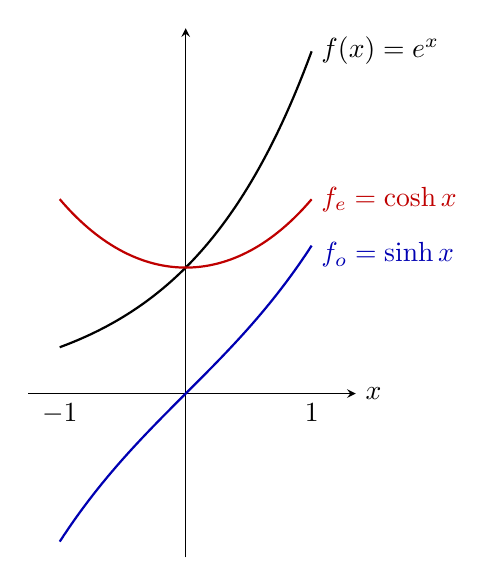
\begin{tikzpicture}[scale=1.6, >=stealth]
\draw[->] (-1.25,0) -- (1.35,0) node[right] {$x$};
\draw[->] (0,-1.3) -- (0,2.9);
\draw[thick, domain=-1:1, samples=60] plot (\x, {exp(\x)});
\draw[thick, red!75!black, domain=-1:1, samples=60] plot (\x, {cosh(\x)});
\draw[thick, blue!70!black, domain=-1:1, samples=60] plot (\x, {sinh(\x)});
\node[right] at (1,2.72) {$f(x) = e^x$};
\node[right, red!75!black] at (1,1.54) {$f_e = \cosh x$};
\node[right, blue!70!black] at (1,1.1) {$f_o = \sinh x$};
\node[below] at (-1,0) {$-1$};
\node[below] at (1,0) {$1$};
\end{tikzpicture}
